\documentclass[sigconf,anonymous]{acmart}

% FPGA 2027 uses the ACM SIGCONF format and double-blind review.
% Keep the official acmart layout unchanged for submission.
\usepackage{booktabs}
\usepackage{multirow}
\usepackage{graphicx}
\usepackage{subcaption}
\usepackage{amsmath}
\usepackage{siunitx}
\usepackage{xspace}
\usepackage{enumitem}
\usepackage{xcolor}

\newcommand{\sys}{\textsc{SCOPE}\xspace}
\newcommand{\tax}{\emph{peripheral integration tax}\xspace}
\newcommand{\TODO}[1]{\textcolor{red}{[TODO: #1]}}

\acmConference[FPGA '27]{The 35th ACM/SIGDA International Symposium on Field-Programmable Gate Arrays}{March 14--16, 2027}{Monterey, CA, USA}
\acmYear{2027}
\copyrightyear{2027}
\settopmatter{printacmref=false}

\hypersetup{
  pdftitle={SCOPE: A Software-Defined Peripheral Subsystem for FPGA Prototyping},
  pdfauthor={Anonymous Authors}
}

\begin{document}

\title{SCOPE: A Software-Defined Peripheral Subsystem for FPGA Prototyping}
\author{Anonymous Author(s)}

\begin{abstract}
FPGA prototypes must run production operating systems and drivers against real
peripherals, yet the devices available to a design under test (DUT) are usually
fixed by board connectors, host placement, and device-specific FPGA logic.
Remote access alone does not solve this problem: an unmodified DUT software
stack must still discover a legal PCIe topology, issue native register and queue
operations, expose DMA buffers, and observe ordered completions. We present
\sys, a software-defined peripheral subsystem that makes the DUT-visible device
composition and backend binding software decisions. \sys realizes this ability
through two architectural separations. It decouples device presentation from
backend implementation and deployment, and separates programmable control
mediation from bulk data movement. A generic FPGA front-end serves a shadowed
configuration hierarchy, routes BAR accesses, transports control events, and
injects interrupts. A host software back-end owns the authoritative topology
and device state, translates device-specific submission semantics and DMA
addresses, and binds each logical endpoint to a physical backend. Coherence
rules across configuration, routing, DMA visibility, and completion preserve
the native device contract after these functions are separated. Our prototype
exposes multiple NVMe endpoints and an Intel NIC to a RISC-V SoC prototype and
runs unmodified Linux NVMe and \texttt{igb} drivers. Initial measurements show
comparable 128-KiB sequential-read throughput for host-attached and on-board
NVMe backends (13.52 versus 13.28 MiB/s) while identifying control mediation and
the low-frequency DUT as the present performance limits.
\end{abstract}

\ccsdesc[500]{Hardware~Reconfigurable logic and FPGAs}
\ccsdesc[300]{Computer systems organization~System on chip}
\ccsdesc[300]{Software and its engineering~Device drivers}

\keywords{FPGA prototyping, PCIe, real peripherals, software-defined I/O, device virtualization}

\maketitle

\section{Introduction}
\label{sec:intro}

FPGA prototypes allow hardware and system software to evolve before silicon is
available. Their value increasingly depends on running a complete software
stack, including the operating system, production drivers, and realistic I/O
workloads. Such validation requires real NVMe SSDs, NICs, and accelerators:
software device models are configurable and observable, but their usefulness is
bounded by the fidelity of the modeled controller, firmware, timing, and DMA
behavior.

Attaching a real device retains its controller and firmware as participants in
validation, but usually makes the
validation environment rigid. The DUT can use only devices reachable through
the prototype board and its host topology. Adding device types often requires
device-specific RTL for configuration, register access, DMA, and interrupts.
Changing the device composition may require rewiring, additional PCIe hardware,
or a new FPGA build. These costs consume both scarce FPGA resources and
engineering time. We call their incremental cost the \tax.

Moving a device to another host does not by itself remove this coupling. A DUT
does not consume an abstract remote-I/O service. Its unmodified Linux stack
expects a locally discoverable PCIe function with coherent configuration and
BAR state. Its driver creates protocol-specific queues, publishes DMA addresses,
rings doorbells, and assumes that data is visible before a completion or
interrupt arrives. Forwarding MMIO operations without preserving this end-to-end
contract may enumerate a device but cannot make it usable.

This paper asks: \emph{Can the peripheral subsystem visible to an FPGA-hosted
DUT be defined in software, without moving complete device implementations into
the FPGA and without changing the DUT driver?} We answer with \sys, a
software-defined peripheral subsystem for FPGA prototyping. ``Software-defined''
has a precise meaning in \sys: within a hardware-supported capacity, software
selects which logical endpoints the DUT sees, binds them to local or remote
physical backends, and chooses how their control semantics and DMA paths are
realized. The bitstream provides stable mechanisms rather than a fixed device
composition.

The design balances two objectives of peripheral access. Virtualization gives
the user control over the logical device view and backend binding. Passthrough
retains execution by a physical controller, including the firmware and I/O
effects exercised by the workload. These objectives meet at a semantic
boundary: a configurable endpoint still has to issue commands that its backend
can execute, and an adapter can alter the timing and behavior observed by the
driver. \sys uses selective mediation to preserve this boundary, with
functional fidelity and timing fidelity treated as distinct validation goals.

\sys obtains this ability through \emph{dual decoupling}. First,
\emph{device-presentation--backend-implementation decoupling} separates the
PCIe identity and driver-visible behavior presented to the DUT from the
physical device's location and backend realization. Second,
\emph{control-semantics--data-path decoupling} allows software to mediate
configuration and runtime control while bulk data uses a separately optimized
DMA path. These separations create flexibility, but they are safe only if the
resulting distributed state still behaves like one device. \sys therefore
enforces three coherence relations: configuration writes become visible
together with their BAR routes; a submission reaches a backend only after its
queue entry and translated DMA addresses are visible; and a completion becomes
visible only after its data effects.

The FPGA front-end implements standard ECAM access, a configuration shadow,
BAR routing, a control-event transport, DMA windows, and interrupt injection.
The host software back-end owns the logical topology and device state, dispatches
accesses by logical BDF, translates NVMe and NIC queue semantics, and connects
each endpoint to a physical device. This partition keeps latency-critical,
interface-facing mechanisms in hardware while placing extensible device
semantics in software.

This paper makes three contributions:
\begin{itemize}[leftmargin=*]
    \item It defines a software-defined peripheral subsystem that turns the
    DUT-visible device composition and endpoint-to-backend binding into software
    configuration rather than a consequence of physical attachment.
    \item It presents a hardware/software architecture based on device-
    presentation--backend-implementation decoupling and control-semantics--
    data-path decoupling, with explicit coherence rules spanning enumeration,
    runtime control, DMA address translation, completion, and interrupts.
    \item It demonstrates the design on a RISC-V SoC FPGA prototype with real
    NVMe and Intel Ethernet backends, and evaluates native-driver compatibility,
    control overhead, data-path performance, and completion/interrupt ordering.
\end{itemize}

The current implementation targets pre-silicon FPGA prototyping. The same
logical abstraction may be useful in post-silicon validation, but we treat that
extension as future work rather than a demonstrated contribution.
Section~\ref{sec:overview} develops the architectural separation,
Section~\ref{sec:design} derives the mechanisms that preserve device semantics,
and Section~\ref{sec:evaluation} evaluates their compatibility and cost.
Section~\ref{sec:discussion} examines the resulting configurability--fidelity
tradeoff.

\section{Background and Motivation}
\label{sec:motivation}

\subsection{Why Real Peripherals Matter}

Full-system validation exercises more than a register specification. An NVMe
driver allocates submission and completion queues, constructs PRP lists, rings a
doorbell, waits for DMA and then consumes a phase-tagged completion. A NIC driver
programs descriptor rings, transfers ownership with queue-tail registers, and
interprets device-specific interrupt causes. Controller firmware, reset corner
cases, DMA ordering, and the interaction with an unmodified driver all affect
the observed behavior. A software model is useful for early bring-up and fault
injection, but every modeled behavior is also an assumption. A physical backend
provides an independent implementation of the device data plane and firmware.

\subsection{Why Physical Attachment Is Insufficient}

Conventional attachment couples three decisions that validation engineers need
to vary independently:
\begin{enumerate}[leftmargin=*]
    \item \textbf{Presentation:} which topology, identities, BARs, and
    capabilities the DUT discovers;
    \item \textbf{Control realization:} where configuration and
    protocol-specific control semantics execute;
    \item \textbf{Data realization:} how a device reaches DUT memory and how
    data and completions return.
\end{enumerate}
The board topology commonly fixes all three. PCIe extension and disaggregation
can move the physical device, but do not automatically synthesize the DUT-facing
topology or translate guest DMA addresses and device semantics. SCOPE therefore
defines the software-configurable boundary narrowly: the FPGA bitstream provides
the generic ECAM, route, mailbox, DMA-window, and interrupt mechanisms, while a
startup backend configuration selects the active endpoints and their bindings.
This is configuration-only composition within a pre-provisioned hierarchy, not
arbitrary runtime hot-plug or an unlimited number of physical devices.

\subsection{The Peripheral Integration Tax}

We define the \tax as the incremental hardware and engineering cost of adding a
device type or instance to an FPGA validation platform. It includes device-
specific RTL, configuration state, on-chip buffers, routing pressure, timing
closure risk, and resynthesis effort. Two axes matter. A new \emph{type} may
require new protocol state machines, whereas another \emph{instance} requires
more addressable state and routing capacity. No implementation can make the
second cost zero. Our goal is narrower: keep the FPGA-side per-instance cost to
generic state and routing entries, and move device-specific state growth to the
software back-end.

\subsection{Requirements}

Four requirements follow. First, an unmodified DUT OS must enumerate and bind
its native driver. Second, configuration, BAR routing, DMA, completion, and
interrupt state must remain mutually consistent even though different agents
own them. Third, control mediation must not force all payload bytes through the
same software path. Fourth, adding an endpoint within the provisioned capacity
should not require a different DUT interface or bitstream. The last requirement
is an implementation property of the generic mechanisms; it still needs a
capacity sweep before we claim a particular FPGA resource slope. \sys does not
attempt to reproduce a physical PCIe link: it validates the system-software and
device interaction above the link layer, not PHY, LTSSM, DLLP, or electrical
behavior.

\section{System Overview}
\label{sec:overview}

\subsection{Software-Defined Peripheral Subsystem}

\sys presents a logical PCIe hierarchy to the DUT. A logical endpoint has a
virtual BDF, configuration image, BAR routes, interrupt state, and a binding to
a backend. The backend may be a physical function attached to the FPGA host or
reachable through a remote transport. The DUT names only logical resources; it
does not know the host BDF, transport endpoint, or host-side DMA aperture.

Figure~\ref{fig:overview} maps the logical device contract onto the FPGA,
host coordinator, and physical backends. Four mechanisms realize this mapping:
logical topology construction, configuration-space virtualization, endpoint
semantic mediation, and DMA-path realization. The first two determine what the
DUT sees; the latter two make that device operational.

\begin{figure*}[t]
    \centering
    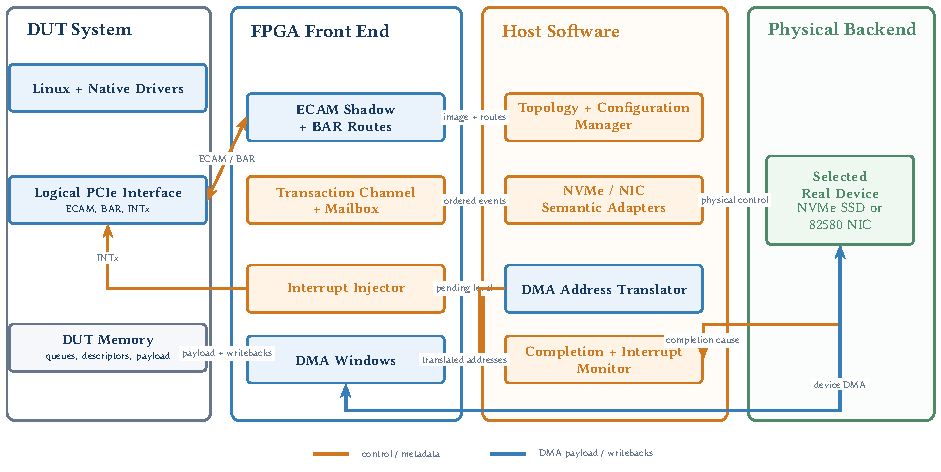
\includegraphics[width=\textwidth]{figures/system_architecture.pdf}
    \caption{\sys architecture. The DUT accesses a logical PCIe interface
    implemented by generic FPGA mechanisms. Host software owns topology and
    device semantics, while a selected physical backend executes device
    operations. Orange arrows carry control and metadata; blue arrows carry DMA
    payload and writebacks without traversing the semantic event channel.}
    \label{fig:overview}
    \Description{A DUT connects through a generic FPGA front-end to host
    coordination software and a real NVMe or Ethernet backend. Control and DMA
    paths are shown separately.}
\end{figure*}

\subsection{Three Planes and the SDN Analogy}
\label{sec:planes}

The architecture separates three responsibilities, following the distinction
between applications, control, and forwarding in software-defined networking
(SDN)~\cite{onf2014architecture}. In \sys, the \emph{software plane} is the
DUT's OS and native drivers, which consume a device interface. The
\emph{control plane} constructs that interface, binds logical endpoints to
backends, and mediates configuration and device control. Its mechanisms span
the FPGA front-end and host coordinator. The \emph{data plane} comprises the
physical backends and the paths through which they exchange payload with DUT
memory. These are functional responsibilities, not three physical machines;
host software in the control plane is distinct from DUT software in the
software plane.

\begin{figure*}[t]
    \centering
    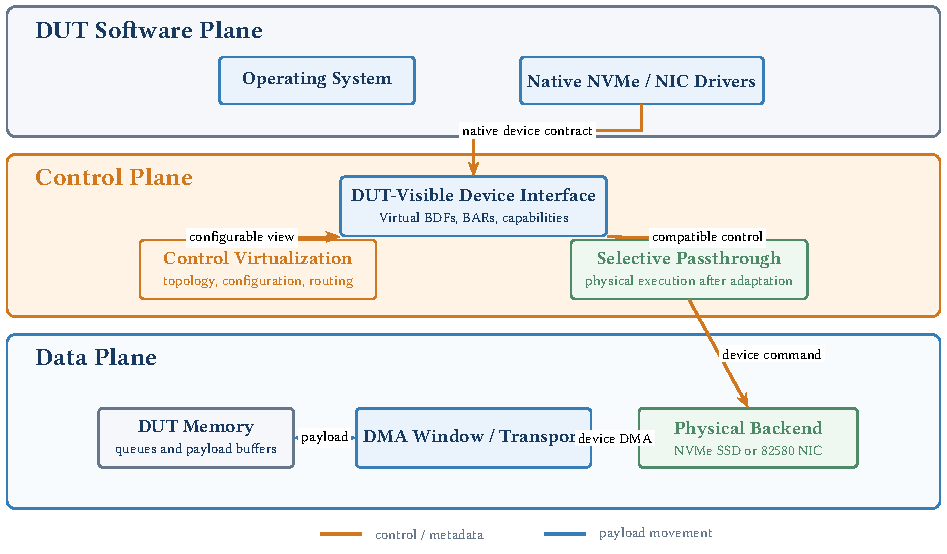
\includegraphics[width=0.92\textwidth]{figures/three_planes.pdf}
    \caption{SDN-inspired separation of peripheral access. Control
    virtualization makes the logical view and binding configurable, while
    selective passthrough retains execution by a physical backend after required
    adaptation. Payload movement follows an independently realized data path.
    Physical execution improves behavioral fidelity for the exposed operations,
    but does not imply direct-attachment timing or PCIe link fidelity.}
    \label{fig:planes}
    \Description{The DUT software plane consumes a virtual device interface.
    The control plane combines virtualization with selective passthrough. The
    data plane connects DUT memory to a real NVMe or Ethernet backend.}
\end{figure*}

The SDN analogy concerns programmable control over a separately realized data
path. The DUT software plane plays the role of a service consumer, but its
interface remains a native device protocol rather than an SDN application API.
The analogy also has a limit: a device submission refers to queues, DMA buffers,
and ownership transitions. Routing an access to the correct backend is
insufficient unless these stateful dependencies remain coherent.

Within the control plane, \emph{control virtualization} creates the logical
configuration and mediates state that differs from the physical backend.
\emph{Control passthrough} retains physical execution of compatible operations,
after any required address or protocol adaptation. The two responsibilities
can coexist for one endpoint. Here passthrough denotes use of the real device,
not transparent forwarding of every register access or full PCIe function
assignment. A direct DMA path is a separate choice: payload can bypass the
software proxy even when submission control is mediated.

\subsection{Dual Decoupling}

Table~\ref{tab:decoupling} separates the two mechanisms. Decoupling device
presentation from backend implementation answers \emph{what device does the DUT see
and which backend implements it?} Control-semantics--data-path decoupling
answers \emph{which operations require semantic mediation and how do payload
bytes move?} Neither alone is sufficient. The first without the second creates
a configurable view whose software proxy may become the data bottleneck. The
second without the first accelerates transfer but leaves device identity and
placement fixed.
The three planes identify responsibilities, whereas dual decoupling identifies
the architectural freedoms between them. The coherence rules below constrain
both freedoms.

\begin{table}[t]
\centering
\caption{Dual decoupling realizes the software-defined abstraction.}
\label{tab:decoupling}
\small
\begin{tabular}{@{}p{0.29\columnwidth}p{0.31\columnwidth}p{0.31\columnwidth}@{}}
\toprule
Mechanism & Separates & Enables \\
\midrule
Device presentation--backend implementation & DUT-visible PCIe identity and behavior from backend placement/realization & Endpoint rebinding, location transparency, software-selected composition \\
Control semantics--data path & Configuration and device control semantics from bulk payload movement & Programmable mediation with independently optimized DMA paths \\
\bottomrule
\end{tabular}
\end{table}

\subsection{Coherence after Separation}

Dual decoupling distributes one device contract across the DUT, FPGA, host
software, and physical backend. \sys restores a single observable order with
three invariants:
\begin{description}[leftmargin=*,style=nextline]
    \item[Configuration--route coherence.] A configuration write completes only
    after the authoritative image and any affected BAR route agree.
    \item[Submission--DMA coherence.] A physical doorbell is issued only after
    the submitted descriptor is stable and every device-visible address has
    been translated to a reachable target.
    \item[Data--completion coherence.] The DUT observes completion state or an
    interrupt only after the corresponding data is visible in DUT memory.
\end{description}
These invariants are not a third decoupling. They constrain the freedom created
by the two separations so the native driver still observes a legal device.

\subsection{Scope of Software Configuration}

The prototype supports a fixed maximum hierarchy and a finite set of generic
route entries. Software activates endpoints, chooses their types, assigns BDFs
under the provisioned switch ports, and binds backends before DUT enumeration.
This is software-configurable composition, not arbitrary online topology
rewiring or PCIe hotplug.

\begin{table}[t]
\centering
\caption{Longer-term access space and the slice evaluated in this paper.}
\label{tab:access-space}
\small
\begin{tabular}{@{}lll@{}}
\toprule
Dimension & Design space & Evaluated slice \\
\midrule
DUT stage & Pre-silicon / post-silicon & Pre-silicon \\
Software access & User / kernel / virtualized & Standard kernel driver \\
Backend placement & Local / remote & Local and host-remote \\
\bottomrule
\end{tabular}
\end{table}

The three dimensions motivate a $2\times3\times2$ design space, but they are
not independent features that the current prototype already implements in all
combinations. We use the table to state the intended abstraction boundary and
the evaluated slice precisely.

\section{Design}
\label{sec:design}

\subsection{Logical Topology Construction}

The software back-end starts from a topology specification that lists enabled
logical endpoints, their virtual BDFs, device templates, and backend bindings.
It constructs Type-1 bridge images and Type-0 endpoint images, including vendor
and device identity, class code, BAR shape, and the capabilities that \sys can
faithfully implement. Capabilities are promises: for example, the current NIC
template omits MSI-X because the prototype implements a shared level interrupt
rather than a virtual MSI-X table and vector remapper.

Topology realization produces two coupled artifacts. A compact ECAM image is
copied into FPGA-visible shadow memory, and a route table maps assigned BAR
ranges to logical backend identifiers. A readiness protocol hides both paths
until the image and routes are initialized, preventing Linux enumeration from
observing a partially constructed hierarchy.

\subsection{Configuration-Space Virtualization}

The FPGA front-end exposes a standard ECAM aperture. Reads to defined BDFs use
the shadow memory fast path; reads to absent functions return all ones. Writes
become fixed-size control events carrying BDF, offset, byte enables, payload,
and a sequence number. Software applies PCI configuration semantics to the
authoritative image, recomputes any BAR route affected by probing or assignment,
writes the changed state back to the shadow, and acknowledges the matching
sequence. Only then does the FPGA complete the DUT write. This rule makes a
subsequent read and BAR access observe the new state.

The shadow is therefore a read cache rather than an independent device model.
Software owns writable semantics, while the FPGA supplies predictable ECAM
latency and a standard interface to the DUT.

\subsection{Endpoint Semantic Mediation}

For runtime access, the FPGA matches a BAR address against its route entries and
emits an event tagged with logical BDF, BAR, offset, width, byte enables, and
sequence. The generic manager dispatches the event to a per-type semantic
adapter. Reads return a value and status through a mailbox. Ordinary writes can
be acknowledged after the required backend effect. Submission writes require a
stronger ordering rule.

A native driver prepares commands or descriptors in memory before writing a
doorbell. The physical backend cannot consume the original entry because it
contains DUT addresses. The adapter waits until the FPGA has accepted the BAR
write and the associated memory entry is stable, parses the entry, translates
its DMA references, writes the translated form, and only then forwards the
physical doorbell. This sequence preserves ownership transfer without requiring
the DUT driver to understand the proxy.

Device semantics remain explicit. The NVMe adapter understands controller
registers, queue setup, doorbells, PRPs and PRP lists, and phase-tagged CQEs. The
NIC adapter understands ring bases and lengths, descriptor buffer addresses,
tail updates, reset behavior, and interrupt cause/mask registers. Common
dispatch and transport do not make unlike devices semantically interchangeable.

\subsection{DMA Data-Path Realization}

\sys separates address retargeting from byte movement. On submission, a semantic
adapter replaces each DUT physical address with an address reachable by the
selected physical backend. For host-local devices, the translated address can
target a coherent alias of DUT memory through the FPGA DMA aperture, allowing
the physical device to move payload without a software copy. A remote backend
may instead use staging or a transport-specific direct path. Both modes preserve
the same logical endpoint contract even though their performance and copy count
differ.

Completion follows the reverse dependency. The back-end first makes returned
payload and device writebacks visible in DUT memory. It then publishes the
guest-visible completion state, updates the adapter's pending state, and finally
changes the virtual interrupt level. This ordering prevents a driver from being
woken before the data it will consume.

\subsection{Interrupt Virtualization}

The initial prototype exports legacy INTx. Each backend maintains private
pending state, and the manager ORs those states into one aggregate level. A
queue-consumption doorbell, mask update, or reset changes only the owning
backend; the physical line is deasserted only when no backend remains pending.
For the NIC, the adapter also preserves read-clear and set/clear semantics of
the interrupt cause and mask registers. MSI/MSI-X requires per-vector table,
address, and delivery virtualization and is outside the current implementation.

\subsection{Scaling the FPGA Mechanism}

The FPGA contains endpoint-independent mechanisms: one ECAM service path, one
control-event channel, one mailbox, a parameterized route table, DMA windows,
and interrupt injection. Adding another supported endpoint consumes another
configuration slot, route state, and software object, but does not replicate an
NVMe or NIC controller in RTL. Adding a device type primarily extends the
software semantic adapter. The remaining hardware cost is real and must be
measured; the intended hypothesis is that it grows with generic capacity rather
than with duplicated device protocol engines. The 1/2/4/8/13-slot synthesis
sweep in Section~\ref{sec:evaluation} is the experiment that can turn this
hypothesis into a quantitative scalability claim.

\section{Implementation}
\label{sec:implementation}

We implement \sys around a RISC-V SoC FPGA prototype running Linux and a host
running a modified QEMU device manager. The FPGA and host communicate through a
Xilinx XDMA endpoint. The current logical hierarchy contains two common bridge
functions and up to thirteen downstream-port/endpoint pairs. Software stores 28
configuration-function slots of 4 KiB each in a compact ECAM shadow; a 128-KiB
dual-port BRAM aperture accommodates the image. The DUT accesses a 16-MiB PCI
memory window in which Linux allocates endpoint BARs.

\subsection{FPGA Front-End}

The front-end implements ECAM decoding, direct shadow reads, serialized
configuration writes, and BAR matching. Configuration and BAR events use
32-byte records carried to a host-allocated cyclic DMA ring. A mailbox carries
acknowledgments, BAR read data, route updates, readiness state, and the aggregate
INTx level in the reverse direction. The XDMA bypass interface exposes both raw
DUT memory and a coherent alias used by physical devices and QEMU when reading
or patching queues.

The virtual hierarchy intentionally stops above the PCIe link. Linux uses the
generic ECAM host bridge, while \sys implements neither a physical downstream
link nor PHY, LTSSM, DLLP, or complete TLP behavior.

\subsection{Software Back-End}

The manager owns the XDMA descriptors, compact ECAM image, route table, and
shared interrupt level. Each endpoint object stores its type, virtual BDF,
backend binding, operations table, and private protocol state. Dispatch by BDF
prevents queue, doorbell, and completion state from leaking between endpoints.
Startup fails atomically if any enabled physical backend cannot be acquired,
preventing a logical endpoint from advertising a device that software cannot
operate.

\subsection{NVMe Adapter}

The NVMe adapter maps a physical controller BAR and virtualizes CAP, VS, CC,
CSTS, queue configuration, and doorbells. It maintains independent queue and
command state per endpoint. Before forwarding a submission doorbell, it reads
the DUT SQE through the coherent alias until two consecutive copies agree,
checks basic field validity, and translates metadata, PRP1, PRP2, and any PRP
list entries. Physical CQEs arrive through the same coherent path. The adapter
validates phase, SQ identifier, head, and outstanding command state before
advancing the guest-visible completion and aggregate interrupt.

\subsection{Ethernet Adapter}

The Ethernet adapter binds one Intel 82580 function to one logical endpoint. It
exposes a 512-KiB BAR0 with device ID \texttt{8086:150e} and class
\texttt{020000}. The virtual capability list hides MSI/MSI-X and BAR3, so the
unmodified Linux \texttt{igb} driver selects one legacy TX/RX queue pair. The
adapter shadows queue-0 ring bases and lengths, rewrites descriptor buffer
addresses, forwards TDT/RDT only after descriptor translation, polls physical
writebacks and causes, and emulates virtual ICR/IMS semantics. Controlled reset
stops DMA, masks the physical device, waits for reset, and clears only that
endpoint's virtual state.

\subsection{Current Boundaries}

The implementation supports BAR0-only endpoints and aggregate INTx. It does not
yet support MSI/MSI-X, AER, hotplug, arbitrary switch capabilities, or multiple
NIC queues. Backend configuration occurs before DUT enumeration. These limits
define the claims and experiments in this paper.

\section{Evaluation}
\label{sec:evaluation}

We organize the evaluation around four questions: (1) can software change the
DUT-visible subsystem without changing its bitstream, (2) do native drivers
remain functional, (3) what control and data overhead does mediation introduce,
and (4) how does provisioned endpoint capacity affect FPGA cost?

\subsection{Experimental Setup}

The DUT is a XiangShan RISC-V SoC prototype running Linux at 50 MHz. The host
communicates with the front-end through XDMA and runs the \sys QEMU back-end.
The evaluated devices include physical NVMe SSDs and an Intel 82580 Ethernet
function. NVMe uses Linux \texttt{fio}; network validation uses DHCP, ping, and
\texttt{iperf}. \TODO{Add FPGA board/part, host CPU, Linux/QEMU versions, XDMA
version, exact device models, link widths/speeds, fio parameters, iperf version,
run count, and error bars.}

\subsection{Software-Defined Composition and Compatibility}

With the same physical wiring and FPGA image, changing only the backend
configuration exposes different populated endpoint sets under the fixed switch
capacity. For each configuration, Linux discovers the bridges and endpoints,
assigns BAR addresses, binds its unmodified \texttt{nvme} or \texttt{igb}
driver, and issues I/O through standard applications. The NVMe path completes
queue initialization and \texttt{fio} traffic. The NIC path reaches physical
link and carrier, completes DHCP in both directions, installs the lease, and
passes bidirectional ping. These results establish a stronger property than
enumeration: configuration, control, translated DMA, completion, and interrupt
handling form a working loop.

\TODO{Add a table whose rows are tested software configurations and whose
columns report topology, backend location, driver bind, initialization, and
workload result. Include an NVMe+NIC simultaneous run to demonstrate composition
rather than isolated device support.}

\subsection{Control-Path Overhead}

Table~\ref{tab:control} separates a basic BAR write from an effective submission
that includes device-specific preparation before the physical doorbell. Host-
mediated control takes tens of microseconds. The submission path costs more than
a simple write because the adapter waits for stable queue memory, translates
DMA references, and preserves the submission ordering invariant.

\begin{table}[t]
\centering
\caption{Measured host-mediated control latency from the current experiment.}
\label{tab:control}
\begin{tabular}{@{}lrr@{}}
\toprule
Device & BAR write (\si{\micro\second}) & Effective doorbell (\si{\micro\second}) \\
\midrule
NVMe & 30.15 & 61.41 \\
Intel NIC & 6.20 & 44.42 \\
\bottomrule
\end{tabular}
\end{table}

\TODO{Define both latency endpoints precisely, reconcile these wall-clock
measurements with the cycle-count results in the presentation, add distributions
and repetitions, and decompose FPGA transport, QEMU dispatch, semantic
translation, and physical BAR access.}

\subsection{End-to-End NVMe Performance}

Table~\ref{tab:nvme} compares two physical placements already measured through
the DUT. Sequential throughput is close: the on-board path reaches 98.2\% of the
host-attached sequential-read result and slightly exceeds its sequential-write
result. Random-read IOPS are also close. Random-write results vary substantially
and require repeated trials before supporting a general claim.

\begin{table}[t]
\centering
\caption{Initial NVMe results observed by the DUT.}
\label{tab:nvme}
\begin{tabular}{@{}lrr@{}}
\toprule
Workload & Host-attached & On-board \\
\midrule
128-KiB sequential read (MiB/s) & 13.52 & 13.28 \\
128-KiB sequential write (MiB/s) & 12.34 & 12.91 \\
4-KiB random read (IOPS) & 176.41 & 174.50 \\
4-KiB random write (IOPS) & 140.62 & 178.07 \\
\bottomrule
\end{tabular}
\end{table}

At 50 MHz and queue depth one, end-to-end throughput is dominated by the slow
DUT and its software submission path. The current data show that tens of
microseconds of control mediation do not dominate these particular workloads;
they do not establish that the overhead will remain hidden for a faster DUT or
higher queue depth. \TODO{Add block-size and queue-depth sweeps, direct-device
baselines, CPU utilization, and repeated measurements with confidence
intervals.}

\subsection{Network Functionality and Performance}

The single-queue NIC backend achieves 56.65 Mbit/s for TCP from the DUT to a
peer and 46.82 Mbit/s in the reverse direction. Measured UDP rates are 4.90 and
7.75 Mbit/s, and ping RTT is 2.80 ms. These values demonstrate a functioning
translated TX/RX path, not line-rate Ethernet. \TODO{Explain the unusually low
UDP results, add loss rate and datagram size, run repeated single-stream TCP
tests, and compare with a direct or on-board NIC baseline.}

\subsection{FPGA Cost and Scaling}

The central hardware claim requires synthesis at multiple provisioned
capacities. \TODO{Report LUT, FF, BRAM/URAM, and Fmax for 1, 2, 4, 8, and 13
endpoint slots; separate fixed front-end cost, configuration-shadow capacity,
and per-route cost. Compare against the earlier single-device proxy or another
FPGA-heavy baseline. Also report RTL changes and resynthesis requirements when
adding the NIC adapter.}

The expected result is not zero per-endpoint cost. Rather, the FPGA slope should
reflect generic configuration and routing capacity, while device-specific queue
and protocol state resides mainly in software. We will state this conclusion
only after the synthesis data are included.

\section{Related Work}
\label{sec:related}

\subsection{FPGA Prototyping Infrastructure}

FASED separates a target DRAM model from its FPGA host implementation and makes
model timing parameters configurable without rebuilding the complete target
\cite{biancolin2019fased}. LEAP provides reusable services and latency-
insensitive interfaces for FPGA applications \cite{fleming2014leap}. RIFFA
offers a portable host--FPGA communication interface \cite{jacobsen2013riffa}.
These systems show the value of stable FPGA infrastructure and host/target
decoupling. \sys applies that principle to a different object: a real
peripheral subsystem that a processor DUT discovers and operates with its
native device driver. Its challenge includes the coupled configuration, BAR,
queue, DMA, completion, and interrupt contract.

\subsection{Modular and Networked FPGA Systems}

Galapagos abstracts heterogeneous CPU/FPGA nodes and makes communication layers
replaceable without changing the application \cite{eskandari2019galapagos}.
Network FPGA clusters similarly separate logical accelerator groupings from
physical datacenter placement \cite{tarafdar2017clusters}. These works organize
compute kernels and their communication. \sys instead organizes devices
presented to an FPGA-hosted processor: the endpoint must participate in PCIe
discovery and preserve a vendor protocol expected by an unmodified OS driver.

\subsection{FPGA Operating Systems and Device Access}

Feniks provides an FPGA OS layer, abstract I/O interfaces, direct PCIe access to
server resources, and a design for remote resource access
\cite{zhang2017feniks}. HybridOS integrates CPU and reconfigurable accelerators
under OS runtime support \cite{kelm2008hybridos}. Their service target is an
FPGA application or accelerator. \sys serves a processor DUT and presents a
driver-compatible device hierarchy. It does not claim remote access or PCIe
peer-to-peer transfer as novel in isolation. Its contribution is the software-
defined endpoint view plus end-to-end mediation needed to take the DUT from
enumeration through native I/O.

\subsection{PCIe Virtualization, Disaggregation, and Composable Fabrics}

Device passthrough and composable PCIe fabrics can assign physical functions or
fabric-attached resources to hosts, and PCIe switches can route those functions
between hosts and devices. Their control plane operates on real PCIe functions
and links; the primary abstraction is resource assignment in the fabric.
\sys instead constructs a logical configuration hierarchy at an FPGA prototype
boundary and may adapt commands and DMA addresses before a physical backend
executes them. Its abstraction is therefore different in two ways: the DUT
sees a software-selected device presentation, and the host coordinator
preserves device-specific control/data semantics across the boundary. \sys is
complementary to composable PCIe hardware, but its evaluation target is
system-software validation rather than transparent extension of the physical
PCIe link.

\subsection{Position of SCOPE}

Across these systems, the reusable idea is a stable interface between a
workload and a changing implementation. SCOPE applies that idea to a processor
DUT that must run a native peripheral driver. The contribution is not a new
PCIe transport, a new NVMe/NIC protocol, or a claim that remote DMA is novel in
isolation. It is the method of combining device-presentation--backend-
implementation decoupling with control-semantics--data-path decoupling, then
constraining the split with configuration--route, submission--DMA, and
data--completion coherence.

\section{Discussion and Limitations}
\label{sec:discussion}

\paragraph{Validation scope.}
\sys validates enumeration, driver initialization, runtime control, DMA, and
interrupt handling against a physical backend. Because it terminates the
DUT-side accesses above the PCIe link, it cannot validate PHY training, LTSSM,
link errors, DLLP/TLP replay, equalization, or electrical behavior. It
complements rather than replaces a physical protocol analyzer or direct-link
test.

\paragraph{Extending device types.}
A new queue-based PCIe device can reuse topology, ECAM, dispatch, and DMA-window
mechanisms, but still needs a semantic adapter that identifies submission
points, translates its DMA-bearing structures, and defines completion ordering.
The NIC experience shows why generic MMIO forwarding is insufficient. A useful
future metric is adapter complexity and the fraction of logic reused across
devices, rather than device count alone.

\paragraph{Performance envelope.}
Software control mediation is appropriate when setup and submission rates are
modest relative to payload work. Faster DUTs, deep queues, or packet-scale
doorbells may expose the tens-of-microseconds path as a bottleneck. Batching,
doorbell coalescing, faster event transport, and selectively moving stable
parsing operations into parameterized hardware are possible responses without
abandoning the overall separation.

\paragraph{Topology and isolation.}
The current system configures a pre-provisioned hierarchy before boot and gives
each physical function to one backend. It does not provide hotplug, arbitrary
switch construction, SR-IOV sharing, malicious-DUT isolation, or live migration.
Those features require explicit IOMMU policy, reset containment, per-vector
interrupt remapping, and failure recovery.

\paragraph{Beyond pre-silicon prototypes.}
The logical subsystem abstraction could also front a fabricated DUT or support
user-space and paravirtual drivers. This produces an attractive longer-term
design space across development stage, driver model, and backend placement.
The present paper does not count those combinations as implemented features;
post-silicon reuse requires a compatible access front-end and separate evidence.

\paragraph{Interpretation of the contribution.}
The central claim is methodological: a stable, software-configurable device
presentation can be separated from backend realization when control semantics
and payload movement are treated as different planes and connected by explicit
coherence rules. The current prototype is evidence for that method in one
pre-silicon slice. MSI/MSI-X, multi-queue operation, AER, hotplug, Vortex/GDS,
post-silicon reuse, and the full $2\times3\times2$ space are extensions, not
unstated results of the present evaluation.

\section{Conclusion}
\label{sec:conclusion}

\sys makes the peripheral subsystem visible to an FPGA-hosted DUT a software
decision. It decouples device presentation from physical implementation and
deployment, and separates programmable control mediation from bulk data
movement. Coherence rules across configuration, routing, submission, DMA data,
completion, and interrupts preserve native device behavior after this split.
The prototype demonstrates that an unmodified Linux stack can enumerate and use
real NVMe and Ethernet backends through a generic FPGA front-end. The remaining
evaluation will quantify the central FPGA claim: that endpoint growth consumes
generic capacity while new device semantics are added primarily in software.


\bibliographystyle{ACM-Reference-Format}
\bibliography{references}

\end{document}
